\section{Software Tasks}
\label{cp4:corpus-tasks}


We start corpus creation by identifying software tasks \gm{for which a 
developer can benefit
from} 
%that require
%a developer to 
foraging information across different artifact \gm{types}. 
We consider a software task as a piece of work undertaken by a developer that often has to be finished within a certain time~\cite{2004merriam}.
\gm{Is there a reference you
could give to a definition
of a software task in 
software? Or can you relate to
a definition in a previous chapter?}


Two common places a software task can be found are:

\begin{itemize}
    \item the description of a \gm{issue
    (e.g., a bug or feature request)} reported in a {issue} tracking system; or in
    \item a post in a community forum, development mailing lists, and others.
\end{itemize}
Several studies have used such  sources for software tasks~\cite{Arya2019, baltes2019, nadi2020, Xu2017}. \gm{Following the lead
of these studies, we select}
GitHub issues and Stack Overflow (SO) posts as sources for potential tasks.

When selecting tasks in GitHub and Stack Overflow, a major challenge arises due to the sheer amount of data available.
Baltes et al.~\cite{baltes2019} argues that even a cursory inspection of a sample set
of Stack Overflow posts shows clear differences in a post's content or structure due to aspects such as programming languages, frameworks, associated technologies, and others.

\gm{To ensure the tasks in the corpus we produce}
%As a means to define a common topic from which we can extract %tasks from each source
%and 
circumvent the heterogeneity of data on GitHub and Stack Overflow, we scope task selection to the \textit{Android} development domain. This decision
restricts task selection to a single programming language (\textit{Java})
while still enabling investigation of a domain that has been
widely discussed by practitioners and researchers alike.
For instance, over 35,000 developers have used Q\&A forums to discuss tasks covering 87\% of the Android API~\cite{parnin2012}
while researchers have investigated how changes to the Android SDK impact its ecosystem and development community~\cite{linares2014, bavota2014b, mcdonnell2013}.


\subsubsection{Stack Overflow tasks}

%Provided that we restrict our corpus to tasks related to %the Android development domain,
We randomly select 150 Stack Overflow posts from a curated list about Android development~\cite{baltes2019-rep}.
\gm{Should you say something about the time period these
tasks are from? Something more about what the curated
list is about? Do you need to argue the tasks are
from different users? I would also start with GitHub tasks
because it is a bit more obvious these are tasks. I think
for Stack Overflow you need to say something about
why these are tasks.}

\gm{I'm a bit confused - is this an example?}
\textit{Saving WebView page to cache}~\cite{so18607655}
is the title of tasks in our corpus extracted from Stack Overflow (Figure~\ref{fig:webview-task}). In this task, a developer describes the need
to
``\textit{save the website the first time it is connected to the internet so that a further connection is no longer needed}''
and their struggle in understanding documentation explaining the WebView component.
To complete this task, a developer will refer to the Android Webview API~\cite{apiWebView}
or Q\&A forums about the Android cache system~\cite{so8410830} so that they can 
formulate a plan with instructions on how to use the API properly.

\begin{figure}
    \centering
    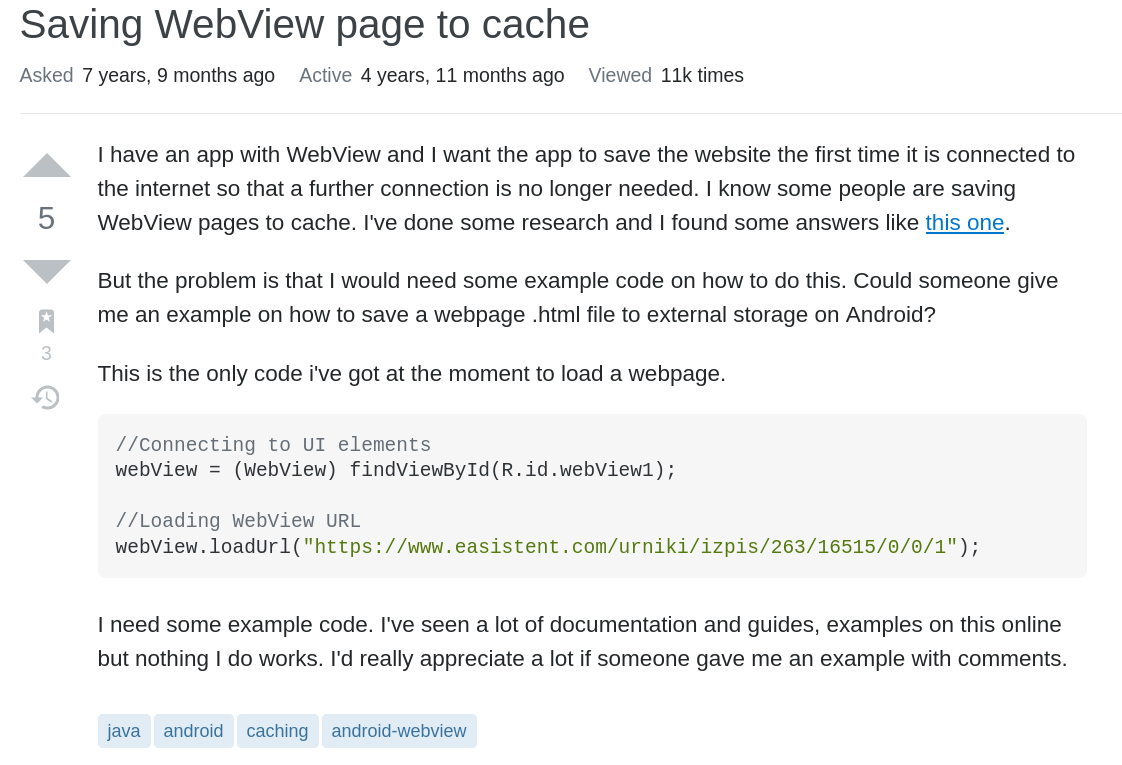
\includegraphics[width=0.85\textwidth]{cp4/webview-task}
    \caption{Sample Stack Overflow task from our corpus}
    \label{fig:webview-task}
\end{figure}

\subsubsection{GitHub tasks}

\gm{To select tasks from GitHub we ...}
%Since we are not aware of a comprehensive dataset of %GitHub issues related to Android development, we %devised our own strategy to fetch such data.
\gm{Can you backup these basic approach with other
papers that use starred projects as a proxy for
popularity?}

We selected 15 top-starred Android projects on GitHub\footnote{\red{info about each project on Appendix}} by filtering the list of projects in the platform to the ones that contained the \textit{Java} and \textit{Android} tags.
For each of these projects, we randomly select 10 issues as the GitHub tasks of our corpus for a total of 150 distinct issues.
While selecting issues, we took care to check that they had at least one follow-up comment and that the issue title did not contain certain words, e.g., {\small \texttt{test}} or {\small  \texttt{ignore}},
so that our selection ignored issues automatically created by scripts or bots---a common pitfall that researchers must be aware of when mining GitHub~\cite{kalliamvakou2014}.



\gm{Is this an example?}
\textit{No lock screen controls ever}~\cite{git3578}
is an example of one of the issues in our corpus extracted from the \texttt{AntennaPod} open-source project (Figure~\ref{fig:lock-screen-task}).
Although the expected behaviour is that the app controls should be visible even with the screen locked,  a user reports that the app screen is missing.
A developer addressing this issue might review the Android lock task documentation~\cite{apiLockTask}
or refer to examples of applications that use the Android lock screen~\cite{mediumLockApp}.
For the remainder of this chapter, we use the lock screen task as a running example.


\begin{figure}
    \centering
    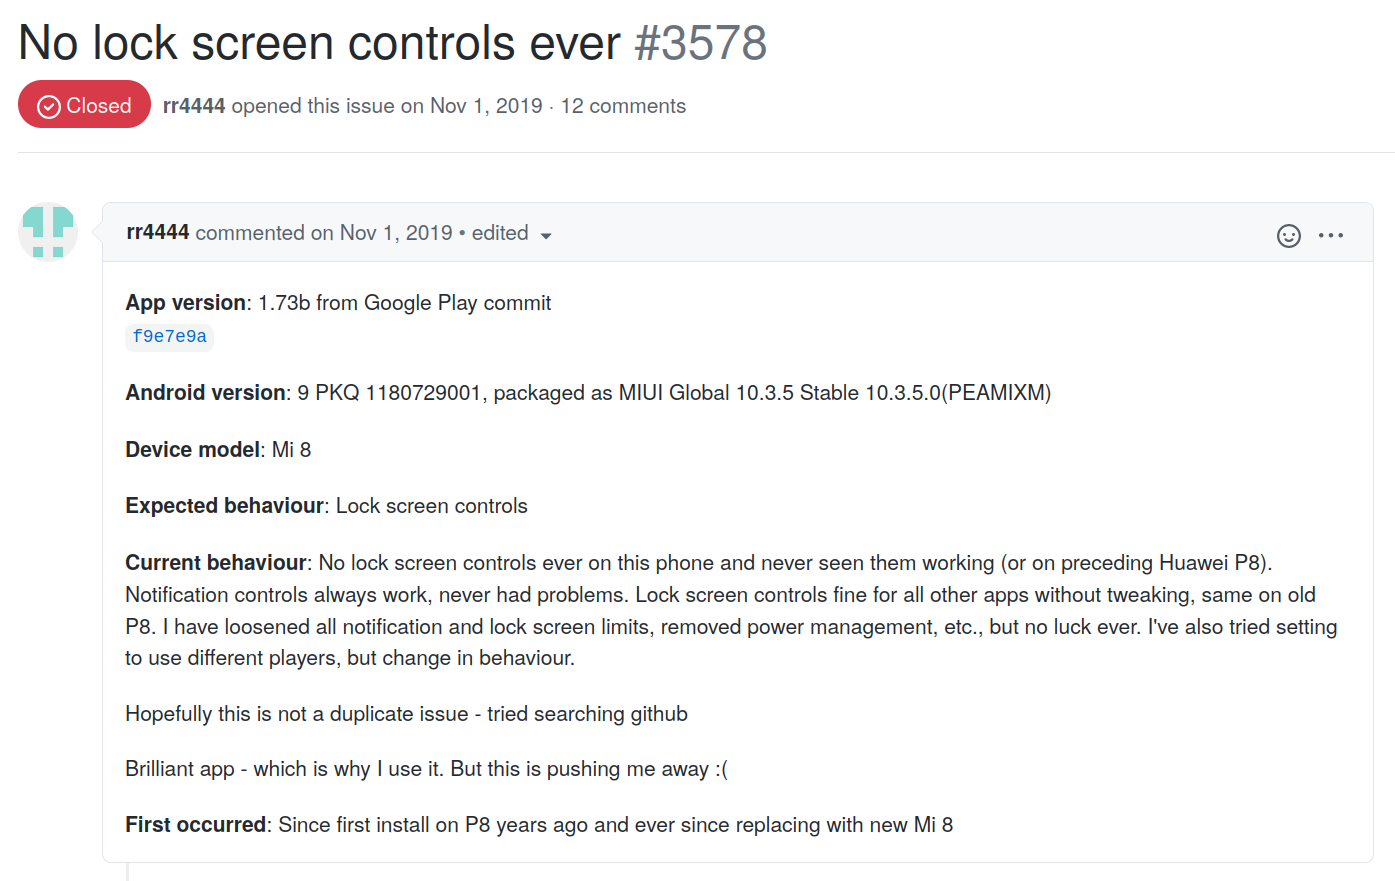
\includegraphics[width=\textwidth]{cp4/lock-screen-task}
    \caption{Sample GitHub task from our corpus}
    \label{fig:lock-screen-task}
\end{figure}